\chapter{DISJOINT SET UNION (DSU)}

\minitoc

\section{Nguồn tài nguyên}

Nội dung bài chủ yếu tham khảo/copy từ [VNOI WIKI] : \url{https://wiki.vnoi.info/algo/data-structures/disjoint-set-union}

\section{Giới thiệu}

\textbf{Disjoint Set Union (DSU)} hay còn gọi là Cấu trúc tập hợp rời rạc, là một cấu trúc dữ liệu rất hữu ích và thường xuyên được sử dụng trong các bài toán lập trình thi đấu.

Đúng như tên gọi, DSU giúp chúng ta quản lý hiệu quả các tập hợp mà không có phần tử chung, và hỗ trợ nhanh các thao tác như:
\begin{itemize}
    \item Kiểm tra xem hai phần tử có nằm trong cùng một tập hay không
    \item Gộp hai tập thành một tập mới
\end{itemize}

\section{Bài toán}

Cho một đồ thị có $n$ đỉnh, ban đầu không có cạnh nào. Chúng ta phải xử lý các truy vấn như sau:

\begin{itemize}
    \item Thêm một cạnh giữa đỉnh $x$ và đỉnh $y$ trong đồ thị.
    \item In ra \texttt{YES} nếu như đỉnh $x$ và đỉnh $y$ nằm trong cùng một thành phần liên thông. In ra \texttt{NO} nếu ngược lại.
\end{itemize}

Một thành phần liên thông trong đồ thị là một đồ thị con trong đó giữa bất kỳ hai đỉnh nào đều có đường đi đến nhau, và không thể nhận thêm bất kỳ một đỉnh nào mà vẫn duy trì tính chất trên.

\subsection{Cấu trúc dữ liệu Disjoint Set Union}

Nếu ta coi mỗi đỉnh trong đồ thị là một phần tử và mỗi thành phần liên thông trong đồ thị là một tập hợp, truy vấn thứ nhất sẽ trở thành gộp hai tập hợp lại thành một và truy vấn thứ hai trở thành hỏi hai phần tử $x$ và $y$ có nằm trong cùng một tập hợp hay không.

Để giải bài toán này, ta sẽ xây dựng một cấu trúc dữ liệu cơ bản thao tác như sau:
\begin{itemize}
    \item \texttt{make\_set(v)}: tạo ra một tập hợp mới chỉ chứa phần tử $v$.
    \item \texttt{union\_sets(a, b)}: gộp tập hợp chứa phần tử $a$ và tập hợp chứa phần tử $b$ thành một.
    \item \texttt{find\_set(v)}: cho biết \textbf{đại diện} của tập hợp có chứa phần tử $v$. Đại diện này sẽ là một phần tử của tập hợp đó và có thể thay đổi sau mỗi lần gọi thao tác \texttt{union\_sets}. Ta sẽ dựa vào đại diện để kiểm tra hai phần tử có nằm trong cùng một tập hợp hay không.
\end{itemize}

Ta có thể xử lý các thao tác này hiệu quả nhờ biểu diễn các tập hợp dưới dạng các cây, mỗi phần tử là một đỉnh và mỗi cây tương ứng với một tập hợp. Gốc của mỗi cây sẽ là đại diện của tập hợp đó.

\begin{figure}[h]
    \centering
    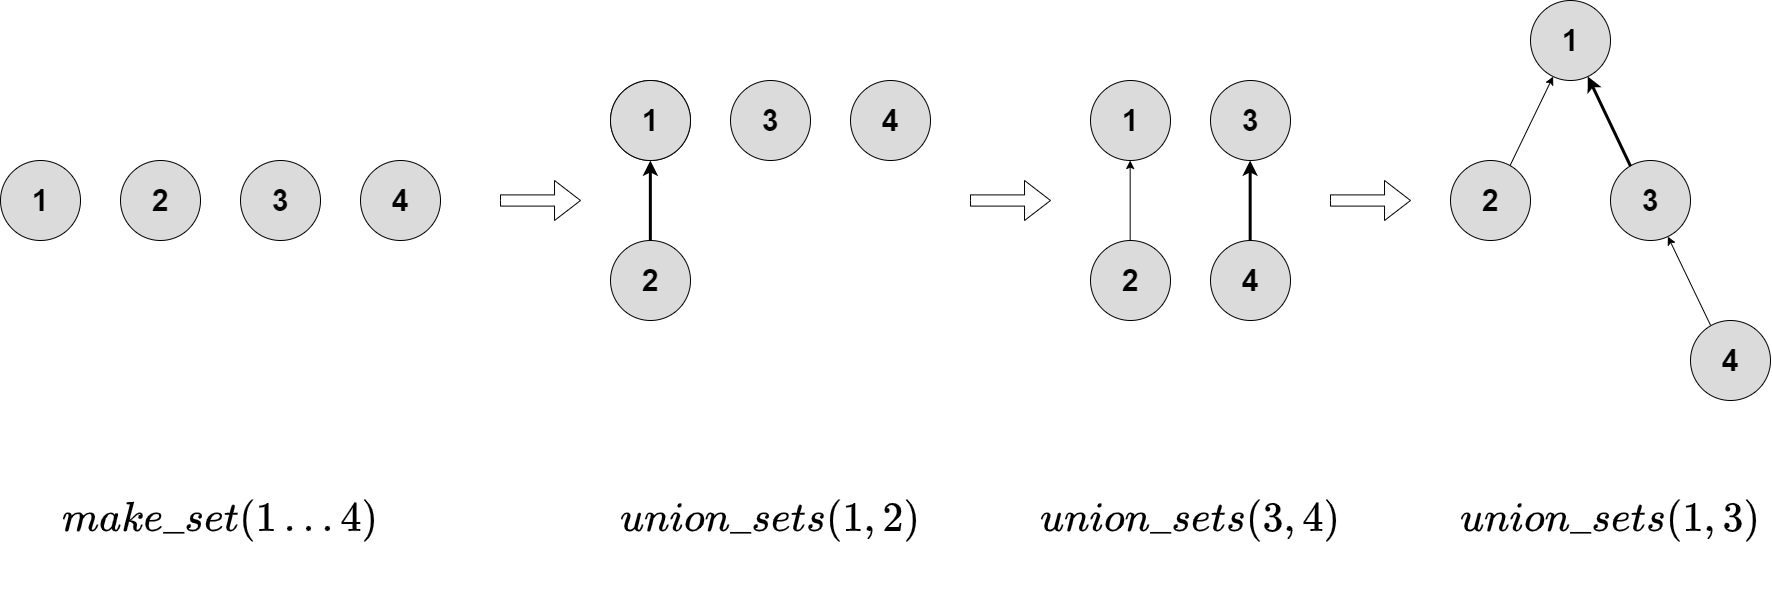
\includegraphics[width=0.7\textwidth]{resource/img/b8/disjoint-set-union_img1.png}
\end{figure}

Ví dụ:
\begin{itemize}
    \item Ban đầu, mỗi phần tử thuộc một tập hợp riêng biệt, vậy mỗi đỉnh là một cây riêng biệt (\texttt{make\_set(1...4)}).
    \item Bước tiếp theo, gộp hai tập hợp chứa phần tử 1 và 2 (\texttt{union\_sets(1,2)}).
    \item Sau đó, gộp hai tập hợp chứa phần tử 3 và 4 (\texttt{union\_sets(3,4)}).
    \item Cuối cùng, gộp hai tập hợp chứa phần tử 1 và 3 (\texttt{union\_sets(1,3)}).
\end{itemize}

Với cách cài đặt này, ta sẽ lưu một mảng \texttt{parent} với \texttt{parent[v]} là cha của phần tử $v$.


\subsection*{Cài đặt ``ngây thơ''}

Để tạo một tập hợp mới gồm phần tử $v$ (hay \texttt{make\_set(v)}), ta chỉ cần tạo một cây có gốc là $v$, với \texttt{parent[v] = v}.

Để gộp hai tập hợp lần lượt chứa phần tử $a$ và phần tử $b$ (hay \texttt{union\_sets(a, b)}), ta sẽ tìm gốc của cây có chứa phần tử $a$ và gốc của cây có chứa phần tử $b$. Nếu hai giá trị này giống nhau, ta sẽ không làm gì do hai phần tử này đã nằm trong cùng một tập hợp. Còn nếu không, ta sẽ đặt gốc cây này là cha của gốc cây còn lại. Dễ thấy điều này sẽ gộp hai cây lại thành một.

Để tìm kí hiệu của một tập hợp có chứa phần tử $v$ (hay \texttt{find\_set(v)}), ta đơn giản nhảy lên các tổ tiên của đỉnh $v$ cho đến khi ta đến gốc của cây. Thao tác này có thể dễ dàng được cài đặt bằng đệ quy.

\begin{lstlisting}[language=C++]
void make_set(int v) {
    parent[v] = v; 
}

int find_set(int v) {
    if (v == parent[v]) return v;
    return find_set(parent[v]); 
}

void union_sets(int a, int b) {
    a = find_set(a);
    b = find_set(b);
    if (a != b) parent[b] = a;
}
\end{lstlisting}

Như đã nói, đây là cách cài đặt ngây thơ, ta có thể dễ dàng tạo ra một ví dụ sao cho khi sử dụng cách cài đặt này, cây sẽ trở thành một đoạn thẳng gồm $n$ phần tử. Trong trường hợp này, độ phức tạp của thao tác \texttt{find\_set} sẽ là $\mathcal{O}(n)$.

Điều này đương nhiên là không thể chấp nhận được, vì vậy ta sẽ tìm hiểu hai phương pháp tối ưu thuật toán dưới đây.

\subsection*{Tối ưu 1 -- Gộp theo kích cỡ / độ cao}

Phương pháp tối ưu này sẽ thay đổi thao tác \texttt{union\_sets}. Ta sẽ thay đổi cách xét trong hai cây đang gộp, gốc của cây nào sẽ là cha của gốc của cây còn lại.

Có hai cách sử dụng phổ biến nhất:
\begin{itemize}
    \item Gộp theo kích cỡ: gốc của cây lớn sẽ là cha của gốc cây nhỏ.
    \item Gộp theo độ cao: gốc của cây có độ cao lớn hơn sẽ là cha của gốc cây có độ cao nhỏ hơn.
\end{itemize}

\paragraph{Gộp theo kích cỡ:}
\begin{lstlisting}[language=C++]
void make_set(int v) {
    parent[v] = v;
    sz[v] = 1;
}

void union_sets(int a, int b) {
    a = find_set(a);
    b = find_set(b);
    if (a != b) {
        if (sz[a] < sz[b]) swap(a, b);
        parent[b] = a;
        sz[a] += sz[b];
    }
}
\end{lstlisting}

\paragraph{Gộp theo độ cao:}
\begin{lstlisting}[language=C++]
void make_set(int v) {
    parent[v] = v;
    rank[v] = 0;
}

void union_sets(int a, int b) {
    a = find_set(a);
    b = find_set(b);
    if (a != b) {
        if (rank[a] < rank[b]) swap(a, b);
        parent[b] = a;
        if (rank[a] == rank[b]) rank[a]++;
    }
}
\end{lstlisting}

Chỉ cần sử dụng phương pháp tối ưu này, độ phức tạp của thao tác \texttt{find\_set} sẽ trở thành $\mathcal{O}(\log n)$. Tuy nhiên, ta vẫn còn có thể làm tốt hơn nữa khi kết hợp với phương pháp tối ưu tiếp theo.

\subsection*{Tối ưu 2 -- Nén đường đi}

Phương pháp tối ưu này nhằm tăng tốc thao tác \texttt{find\_set}.

Giả sử ta gọi \texttt{find\_set(v)} với một đỉnh $v$ bất kỳ, chúng ta tìm được $p$ là gốc của cây. Đồng thời, mọi hàm \texttt{find\_set(u)} với $u$ là một đỉnh nằm trên đường đi từ $u$ đến $p$, sẽ trả về $p$. Cách tối ưu ở đây chính là làm cho đường đi đến gốc của các đỉnh $u$ ngắn đi bằng cách gán trực tiếp cha của các đỉnh $u$ này thành $p$.

\begin{figure}[h]
    \centering
    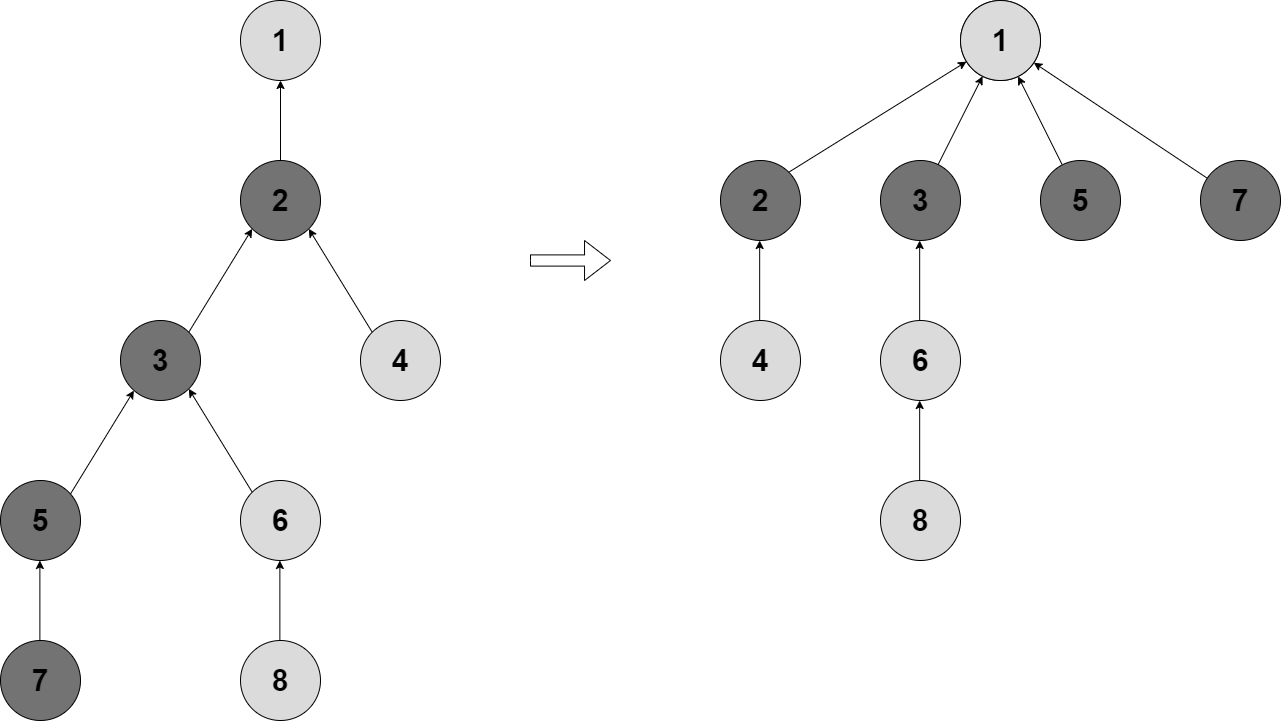
\includegraphics[width=0.6\textwidth]{resource/img/b8/disjoint-set-union_img2.png}
\end{figure}

Sau khi thực hiện tối ưu này, cấu trúc cây có thể thay đổi: các đỉnh nằm trên đường đi đến gốc sẽ nối trực tiếp với gốc.

\paragraph{Cài đặt thao tác \texttt{find\_set} có nén đường đi:}
\begin{lstlisting}[language=C++]
int find_set(int v) {
    if (v == parent[v]) return v;
    int p = find_set(parent[v]);
    parent[v] = p;
    return p;
}
\end{lstlisting}

\paragraph{Hoặc phiên bản ngắn gọn:}
\begin{lstlisting}[language=C++]
int find_set(int v) {
    return v == parent[v] ? v : parent[v] = find_set(parent[v]);
}
\end{lstlisting}

\subsection*{Một cách cài đặt khác: DSU chỉ dùng mảng \texttt{lab[]}}

Ở một số tài liệu như \textit{Giải thuật và lập trình} (thầy Lê Minh Hoàng) hay thư viện Atcoder, cấu trúc DSU (Disjoint Set Union) có thể được cài đặt chỉ với một mảng duy nhất là \texttt{lab[]} thay vì hai mảng \texttt{parent[]} và \texttt{sz[]}.

\textbf{Ý tưởng:}
\begin{itemize}
    \item Nếu \texttt{lab[v]} là một số âm, thì $-lab[v]$ là số lượng đỉnh của cây có gốc $v$ (tức $v$ là gốc của cây).
    \item Nếu \texttt{lab[v]} là một số dương, thì \texttt{lab[v]} chính là cha của $v$.
\end{itemize}

\paragraph{Cài đặt:}
\begin{lstlisting}[language=C++]
void make_set(int v) {
    lab[v] = -1;
}

int find_set(int v) {
    return lab[v] < 0 ? v : lab[v] = find_set(lab[v]);
}

void union_sets(int a, int b) {
    a = find_set(a);
    b = find_set(b);
    if (a != b) {
        if (lab[a] > lab[b]) swap(a, b);
        lab[a] += lab[b];
        lab[b] = a;
    }
}
\end{lstlisting}

\textbf{Giải thích:}
\begin{itemize}
    \item \texttt{make\_set(v)}: Khởi tạo một cây mới gồm phần tử $v$, lúc này $v$ là gốc, và cây có đúng 1 phần tử nên \texttt{lab[v] = -1}.
    \item \texttt{find\_set(v)}: Trả về gốc của cây chứa $v$, đồng thời tối ưu bằng nén đường đi (path compression).
    \item \texttt{union\_sets(a, b)}: Gộp hai cây chứa $a$ và $b$ lại, gốc của cây nhỏ hơn (tức có kích thước lớn hơn về giá trị âm) sẽ nhận cây còn lại. Cụ thể, nếu \texttt{lab[a] > lab[b]} thì hoán vị $a, b$ để luôn gộp cây $b$ vào cây $a$.
    \item Sau khi gộp, cập nhật lại kích thước: \texttt{lab[a] += lab[b]} và gán \texttt{lab[b] = a} (gốc mới của $b$).
\end{itemize}

\section{Một số ứng dụng của DSU}

\subsection*{Lưu thêm thông tin khác cho mỗi tập hợp}

Ngoài việc lưu các thông tin về cấu trúc cây, ta có thể lưu các hàm có tính chất giao hoán và kết hợp của từng tập hợp. Ví dụ, ta có thể lưu tổng các phần tử/giá trị phần tử bé nhất của từng tập hợp. Lúc này, các thao tác của DSU sẽ được cài đặt như sau:

\begin{lstlisting}[language=C++]
void make_set(int v) {
    parent[v] = v;
    sz[v] = 1;
    mn[v] = value[v];
    sum[v] = value[v];
}

int find_set(int v) {
    return v == parent[v] ? v : parent[v] = find_set(parent[v]);
}

void union_sets(int a, int b) {
    a = find_set(a);
    b = find_set(b);
    if (a != b) {
        if (sz[a] < sz[b]) swap(a, b);
        parent[b] = a;
        sz[a] += sz[b];
        sum[a] += sum[b];
        mn[a] = min(mn[a], mn[b]);
    }
}
\end{lstlisting}

Có thể thấy rằng, tương tự như thông tin về độ lớn của cây (\texttt{sz}) hay độ cao của cây (\texttt{rank}), ta sẽ lưu các hàm này tại gốc của từng cây.

\begin{lstlisting}[language=C++]
int find_sum(int v) {
    v = find_set(v);
    return sum[v];
}

int find_min(int v) { 
    v = find_set(v);
    return mn[v];
}
\end{lstlisting}

\section{Bài toán xếp hàng}

\subsection*{Bài toán}

Cho \( n \) người đang xếp hàng ở các vị trí từ 1 đến \( n \). Viết chương trình xử lý các truy vấn:

\begin{itemize}
    \item Người đứng ở vị trí thứ \( i \) rời khỏi hàng.
    \item Tìm người gần nhất về bên phải vị trí \( p \) mà chưa rời khỏi hàng.
\end{itemize}

\subsection*{Lời giải}

Với mỗi vị trí, ta sẽ có một con trỏ. Nếu người đứng ở vị trí này vẫn đang đứng trong hàng, con trỏ trỏ vào vị trí đó, nếu không thì con trỏ này sẽ trỏ vào vị trí ngay bên phải.

Xét ví dụ sau với \( n = 5 \), ban đầu ta có:

\begin{figure}[h]
    \centering
    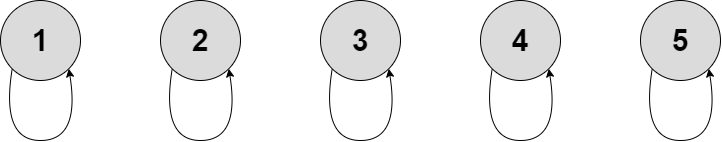
\includegraphics[width=0.5\textwidth]{resource/img/b8/disjoint-set-union_img3.png}
\end{figure}

Giả dụ người đứng ở vị trí 2 và 3 rời khỏi hàng:

\begin{figure}[h]
    \centering
    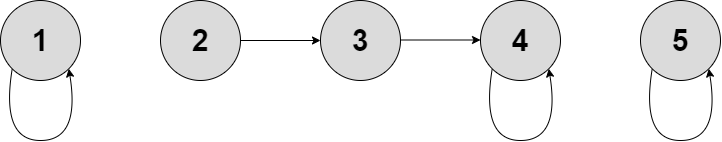
\includegraphics[width=0.5\textwidth]{resource/img/b8/disjoint-set-union_img4.png}
\end{figure}

Ta thấy để tìm người gần nhất bên phải mà chưa rời khỏi hàng, ta đi dần dần sang phải cho đến khi gặp một vị trí có con trỏ đến chính nó.

Chúng ta có thể sử dụng cấu trúc dữ liệu DSU để lưu trữ các thông tin trên và sử dụng phương pháp tối ưu nén đoạn để đạt được độ phức tạp trung bình \(O(\log n)\) với mỗi truy vấn.

Để ý kĩ hơn, ta thấy vị trí ta cần tìm chính là vị trí có thứ tự lớn nhất trong tập hợp. Ta có thể lưu phần tử lớn nhất trong một tập hợp như đã nói ở phần trên, qua đó đạt được độ phức tạp trung bình \(O(\alpha(n))\) với mỗi truy vấn.

%\section*{Code mẫu}
\paragraph{Cài đặt}
\begin{lstlisting}[language=C++]
void make_set(int v) {
    parent[v] = v;
    sz[v] = 1;
    mx[v] = v;
}

int find_set(int v) {
    return v == parent[v] ? v : parent[v] = find_set(parent[v]);
}

void union_sets(int a, int b) {
    a = find_set(a);
    b = find_set(b);
    if (a != b) {
        if (sz[a] < sz[b]) swap(a, b);
        parent[b] = a;
        sz[a] += sz[b];
        mx[a] = max(mx[a], mx[b]);
    }
}

void leave(int v) { 
    union_sets(v, v + 1);
}

int find_next(int p) { 
    p = find_set(p);
    return mx[p];
}
\end{lstlisting}

\begin{baitap}{Path Queries}{https://codeforces.com/contest/1213/problem/G}

Bạn được cho một cây có trọng số gồm $n$ đỉnh. Nhắc lại rằng, cây là một đồ thị liên thông không có chu trình. Đỉnh $u_i$ và $v_i$ được nối với nhau bằng một cạnh có trọng số $w_i$.

Bạn được cho $m$ truy vấn. Truy vấn thứ $i$ là một số nguyên $q_i$. Với truy vấn này, bạn cần tính số cặp đỉnh $(u,v)$ ($u < v$) sao cho trọng số lớn nhất của một cạnh trên đường đi đơn giản giữa $u$ và $v$ không vượt quá $q_i$.

\textbf{Input}

\begin{itemize}
    \item Dòng đầu tiên chứa hai số nguyên $n$ và $m$ ($1 \le n,m \le 2 \cdot 10^5$) — số đỉnh của cây và số truy vấn.
    \item Mỗi dòng trong số $n-1$ dòng tiếp theo mô tả một cạnh của cây. 
    Cạnh thứ $i$ được cho bởi ba số nguyên $u_i, v_i, w_i$ ($1 \le u_i,v_i \le n, u_i \ne v_i$) — nhãn của hai đỉnh mà cạnh nối và trọng số của cạnh ($1 \le w_i \le 2 \cdot 10^5$). 
    Đảm bảo rằng các cạnh đã cho tạo thành một cây.
    \item Dòng cuối chứa $m$ số nguyên $q_1, q_2, \dots, q_m$ ($1 \le q_i \le 2 \cdot 10^5$), trong đó $q_i$ là trọng số cạnh tối đa cho truy vấn thứ $i$.
\end{itemize}

\textbf{Output}

In ra $m$ số nguyên — câu trả lời cho các truy vấn.  

Giá trị thứ $i$ phải bằng số lượng cặp đỉnh $(u,v)$ ($u < v$) sao cho trọng số lớn nhất trên đường đi đơn giản giữa $u$ và $v$ không vượt quá $q_i$.

\textbf{Ví dụ}

\paragraph{Input}
\begin{lstlisting}
7 5
1 2 1
3 2 3
2 4 1
4 5 2
5 7 4
3 6 2
5 2 3 4 1
\end{lstlisting}
\paragraph{Output}
\begin{lstlisting}
21 7 15 21 3 
\end{lstlisting}

\begin{figure}[h]
    \centering
    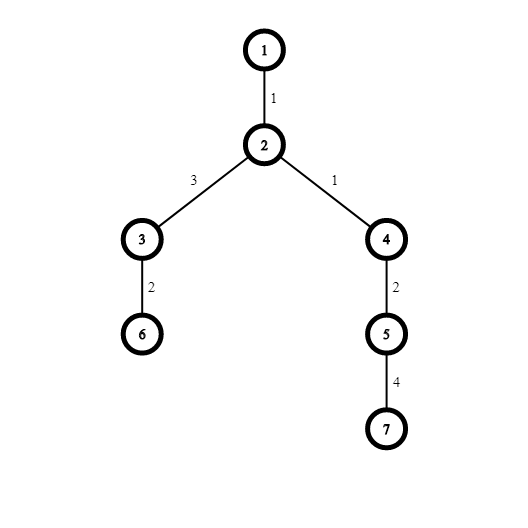
\includegraphics[width=0.4\textwidth]{resource/img/b8/path_queries_1.png}
    \caption{Minh họa ví dụ}
\end{figure}

\end{baitap}

\textbf{Phân tích bài toán}


Giả sử ta đang xét truy vấn với giá trị $q_k$. Khi đó, ta quan tâm đến các thành phần liên thông (TPLT) trong đồ thị chỉ gồm những cạnh có trọng số $\leq q_k$.  

Trong mỗi TPLT, nếu có $e$ đỉnh thì số cặp $(u,v)$ hợp lệ là:
\[
\binom{e}{2} = \frac{e(e-1)}{2}.
\]

Vậy với truy vấn $q_k$, ta chỉ cần tính tổng $\binom{e}{2}$ của tất cả các TPLT sau khi giữ lại các cạnh $\leq q_k$.\\

Để xử lý nhiều truy vấn, ta sắp xếp lại:

\begin{itemize}
    \item Sắp xếp các truy vấn $q_1, q_2, \dots, q_m$ theo thứ tự tăng dần.
    \item Sắp xếp các cạnh của cây theo trọng số tăng dần.
\end{itemize}

Sau đó ta dùng DSU:

\begin{itemize}
    \item Ban đầu, mỗi đỉnh là một TPLT riêng (cỡ $1$).
    \item Khi xét đến cạnh $(u_i, v_i, w_i)$, nếu $w_i \leq q_k$, ta \texttt{union} hai TPLT chứa $u_i$ và $v_i$.
    \item Khi gộp hai TPLT có kích thước $a$ và $b$:
    \begin{itemize}
        \item Trước khi gộp, chúng đóng góp $\binom{a}{2} + \binom{b}{2}$. Sau khi gộp thành TPLT có kích thước $a + b$, ta có $\binom{a + b}{2}$.
        \item Vậy thì phần tăng thêm vào kết quả sẽ là: $\binom{a + b}{2} - \binom{b}{2} - \binom{a}{2}$
    \end{itemize}
\end{itemize}

Bằng cách này, ta duyệt lần lượt các truy vấn (theo thứ tự đã sắp xếp) và thêm dần các cạnh đủ điều kiện, đồng thời cập nhật số cặp hợp lệ.  

Cuối cùng, ta in ra kết quả tương ứng với thứ tự truy vấn ban đầu.

\paragraph{Cài đặt}
\begin{lstlisting}
#include <bits/stdc++.h>
#define int long long
#define endl "\n"
using namespace std;

const int oo = 1e18;
const int MAXN = 100005;

struct Edge {
    int u, v, w;
};

bool compare(const Edge &cur, const Edge &other) {
    return cur.w < other.w;
}

vector<Edge> Graph;
vector<int> parent, sz;
int ans = 0;
int C(int n) {
    return n * (n - 1) / 2;
}

void make_set(int v) {
    parent[v] = v;
    sz[v] = 1;
}

int find_set(int v) {
    if (v == parent[v]) return v;
    int p = find_set(parent[v]);
    parent[v] = p;
    return p;
}

void union_sets(int a, int b) {
    a = find_set(a);
    b = find_set(b);
    if (a != b) {
        if (sz[a] < sz[b]) swap(a, b);
        ans += C(sz[a] + sz[b]) - C(sz[a]) - C(sz[b]);
        parent[b] = a;
        sz[a] += sz[b];
    }
}

signed main() {
    int n, m; cin >> n >> m;
    parent.resize(n + 1); sz.resize(n + 1);
    for (int i = 1; i <= n - 1; i++) {
        Edge cur;
        cin >> cur.u >> cur.v >> cur.w;
        Graph.push_back(cur);
    }
    for (int i = 1; i <= n; i++) {
        make_set(i);
    }

    sort(Graph.begin(), Graph.end(), compare);
    vector<pair<int,int>>q(m + 1);
    for (int i = 1; i <= m; i++) {
        cin >> q[i].first;
        q[i].second = i;
    }

    sort(q.begin() + 1, q.end());

    int idx = 0;
    
    vector<int> res(m + 1);
    for (int i = 1; i <= m; i++) {
        int val = q[i].first;
        while (idx <= n - 2 && Graph[idx].w <= val) {
            union_sets(Graph[idx].u,Graph[idx].v);
            idx++;
        }
        res[q[i].second] = ans;
    }
    for (int i = 1; i <= m; i++) {
        cout << res[i] << " ";
    }
}
\end{lstlisting}

\begin{baitap}{Roads not only in Berland}{https://codeforces.com/contest/25/problem/D}
Chính phủ Berland quyết định cải thiện quan hệ với các quốc gia láng giềng. 
Trước hết, họ quyết định xây dựng các con đường mới để từ mỗi thành phố của Berland và các quốc gia láng giềng có thể đi đến tất cả các thành phố khác. 
Có tổng cộng $n$ thành phố ở Berland và các nước láng giềng, và đúng $n - 1$ con đường hai chiều. 

Do khủng hoảng tài chính gần đây, chính phủ Berland đang rất thiếu tiền, 
nên để xây một con đường mới thì họ phải đóng một con đường hiện tại. 
Mỗi ngày, họ có thể đóng một con đường và ngay lập tức xây một con đường mới. 

Nhiệm vụ của bạn là xác định số ngày ít nhất cần thiết để xây dựng lại các con đường sao cho từ mỗi thành phố có thể đi đến tất cả các thành phố khác, 
và lập kế hoạch đóng đường cũ và xây đường mới.

\textbf{Input}

Dòng đầu tiên chứa số nguyên $n$ ($2 \le n \le 1000$) — số lượng thành phố ở Berland và các quốc gia láng giềng.  

Mỗi dòng trong $n - 1$ dòng tiếp theo mô tả một con đường.  
Mỗi con đường được cho bởi hai số nguyên $a_i, b_i$ ($1 \le a_i, b_i \le n, a_i \ne b_i$) — cặp thành phố mà con đường nối.  

Không thể có nhiều hơn một con đường giữa cùng một cặp thành phố.  
Không có con đường nào nối một thành phố với chính nó.

\textbf{Output}

In ra số $t$ — số ngày ít nhất cần thiết để xây dựng lại các con đường để từ mỗi thành phố có thể đi đến tất cả các thành phố khác.  

Sau đó in $t$ dòng — kế hoạch đóng và mở đường.  
Mỗi dòng mô tả một ngày theo định dạng: 
$
i \; j \; u \; v
$

Điều này có nghĩa là con đường giữa các thành phố $i$ và $j$ bị đóng, và một con đường mới giữa các thành phố $u$ và $v$ được xây.  

Các thành phố được đánh số từ $1$.  
Nếu có nhiều đáp án đúng, bạn có thể in ra bất kỳ đáp án nào.

\textbf{Ví dụ}
\paragraph{Input}
\begin{lstlisting}
7
1 2
2 3
3 1
4 5
5 6
6 7
\end{lstlisting}

\paragraph{Output}
\begin{lstlisting}
1
3 1 3 7
\end{lstlisting}
\end{baitap}

\textbf{Phân tích bài toán.}

Mỗi khi ta xây thêm một con đường mới, mục tiêu là làm giảm số TPLT, tức là nối TPLT $A$ và TPLT $B$ thành một TPLT duy nhất. \\

Ngược lại, khi ta xóa một con đường cũ, yêu cầu là \textit{không được làm tăng số TPLT}. 
Điều này có nghĩa là ta không được phép ``chẻ đôi'' một TPLT hiện có. 
Nói cách khác, để một cạnh có thể bị xóa an toàn, nó phải nằm trên một chu trình trong TPLT: 
khi đó, cạnh này được coi là một cạnh ``dư thừa'' vì việc xóa nó không phá vỡ tính liên thông. \\

Từ đó, ta có chiến lược: 
\begin{itemize}
    \item Với một TPLT $A$, chọn một TPLT $B$ khác (chưa thuộc $A$) và nối chúng lại bằng một cạnh mới.
    \item Đồng thời, trong $A$ (hoặc $B$ sau khi nối), luôn tồn tại ít nhất một cạnh nằm trên chu trình, 
    và ta có thể xóa cạnh ``dư thừa'' này để đảm bảo số cạnh vẫn đúng.
\end{itemize}

Như vậy, mỗi lần ``đóng–mở'' đường ta đều hợp thức: giảm số TPLT đi $1$, 
cho đến khi toàn bộ đồ thị chỉ còn một TPLT duy nhất. \\

\textbf{[Groot]:} Oke, mày lảm nhảm nghe cũng hay đó, nhưng tao vẫn chưa hình dung được cách cài đặt. Kiểu làm sao để cài đặt tìm cạnh dư thừa ấy?

\textbf{[vuivethoima]:} Khi union\_sets$(u, v)$, nếu tụi nó đã nằm cùng một TPLT, thì tức là thêm cạnh $(u, v)$ vào không ảnh hưởng đến việc giảm TPLT. Vậy nó chính là một cạnh dư thừa.

\paragraph{Cài đặt}
\begin{lstlisting}
#include <bits/stdc++.h>
#define int long long
#define endl "\n"
using namespace std;

vector<int> parent(1005), sz(1005);
vector<pair<int,int>> close_edges, new_edges;

void make_set(int v) {
    parent[v] = v;
    sz[v] = 1;
}

int find_set(int v) {
    if (v == parent[v]) return v;
    return parent[v] = find_set(parent[v]);
}

void union_sets(int a, int b) {
    a = find_set(a);
    b = find_set(b);
    if (a != b) {
        if (sz[a] < sz[b]) swap(a, b);
        parent[b] = a;
        sz[a] += sz[b];
    }
}

signed main() {
    int n; cin >> n;
    for (int i = 1; i <= n; i++) make_set(i);

    vector<pair<int,int>> edges;
    for (int i = 1; i < n; i++) {
        int u, v; cin >> u >> v;
        edges.push_back({u, v});
    }

    for (auto [u, v] : edges) {
        if (find_set(u) != find_set(v)) {
            union_sets(u, v);
        } else {
            close_edges.push_back({u, v});
        }
    }

    vector<int> reps;
    for (int i = 1; i <= n; i++) {
        if (find_set(i) == i) reps.push_back(i);
    }

    for (int i = 0; i + 1 < reps.size(); i++) {
        new_edges.push_back({reps[i], reps[i+1]});
        union_sets(reps[i], reps[i+1]);
    }

    cout << close_edges.size() << endl;
    for (int i = 0; i < (int)close_edges.size(); i++) {
        cout << close_edges[i].first << " " << close_edges[i].second << " " 
             << new_edges[i].first << " " << new_edges[i].second << endl;
    }
}
\end{lstlisting}

\begin{baitap}{Mocha and Diana (Easy Version)}{https://codeforces.com/contest/1559/problem/D1}

Một \emph{forest} (rừng) là một đồ thị vô hướng không có chu trình (không nhất thiết phải liên thông).  

Mocha và Diana là bạn bè ở Zhijiang, cả hai đều có một forest với các đỉnh được đánh số từ $1$ đến $n$, và họ muốn thêm các cạnh vào rừng của mình sao cho:  

\begin{itemize}
    \item Sau khi thêm các cạnh, cả hai đồ thị của họ vẫn là forest.
    \item Họ thêm cùng một tập cạnh. Nghĩa là nếu cạnh $(u,v)$ được thêm vào rừng của Mocha thì cạnh $(u,v)$ cũng được thêm vào rừng của Diana, và ngược lại.
\end{itemize}

Mocha và Diana muốn biết số lượng cạnh tối đa mà họ có thể thêm, và những cạnh nào sẽ được thêm.  

\textbf{Input}  

Dòng đầu tiên chứa ba số nguyên $n, m_1, m_2$ $(1 \leq n \leq 1000, 0 \leq m_1, m_2 < n)$ — số lượng đỉnh và số cạnh ban đầu trong rừng của Mocha và Diana.  

Mỗi dòng trong $m_1$ dòng tiếp theo chứa hai số nguyên $u, v$ $(1 \leq u, v \leq n, u \neq v)$ — biểu diễn một cạnh trong rừng của Mocha.  

Mỗi dòng trong $m_2$ dòng tiếp theo chứa hai số nguyên $u, v$ $(1 \leq u, v \leq n, u \neq v)$ — biểu diễn một cạnh trong rừng của Diana.

\textbf{Output}

Dòng đầu tiên in ra một số nguyên $h$, là số cạnh tối đa mà Mocha và Diana có thể thêm (vào mỗi rừng).  

Mỗi dòng trong $h$ dòng tiếp theo in ra hai số nguyên $u, v$ $(1 \leq u, v \leq n, u \neq v)$ — biểu diễn cạnh được thêm vào.  

Nếu có nhiều đáp án đúng, bạn có thể in ra bất kỳ một đáp án nào.

\textbf{Ví dụ}
\paragraph{Input}
\begin{lstlisting}
5 3 2
5 4
2 1
4 3
4 3
1 4
\end{lstlisting}

\paragraph{Output}
\begin{lstlisting}
1
2 4
\end{lstlisting}
\end{baitap}

\textbf{Phân tích bài toán.}

Ta gọi forest của Mocha và Diana lần lượt là $f_1$ và $f_2$.\\

Để không mất tính chất forest, ta xét lần lượt cặp đỉnh $(u, v)$. Nếu $(u, v)$ đều là 2 đỉnh không thuộc cùng một TPLT trong cả $f_1$ và $f_2$, ta chọn $(u, v)$ là cạnh được thêm vào, đồng thời union\_sets$(u, v)$ trong $f_1$ và $f_2$.\\

\textbf{[Groot]:} ê kiểu tao nghe nó ``tham lam'' quá, liệu cứ thêm vô tội vạ như vậy thì liệu kết quả có tối ưu không? Ý tao là tại vì sao mày chắc chắn cái cách làm của mày là đúng, lỡ như thêm $(u,v)$ vào thì sẽ hạn chế các lần thêm sau ấy? Mày hiểu ý tao không??

\textbf{[vuivethoima]:} Ờ dù *éo hiểu câu hỏi của mày cho lắm, nhưng mày thắc mắc vậy là đúng. Nhưng ở đây cái ``tham lam'' này thực ra \textbf{không làm mất đi tối ưu}. Lý do là:

\begin{enumerate}
    \item Một cạnh $(u,v)$ chỉ được chọn nếu nó nối hai TPLT \emph{khác nhau} trong cả $f_1$ lẫn $f_2$.  
    Nghĩa là khi thêm cạnh này, số TPLT trong $f_1$ giảm ít nhất $1$ và số TPLT trong $f_2$ cũng giảm ít nhất $1$.

    \item Vì nó giảm số TPLT đồng thời trong cả hai đồ thị, cạnh này không thể gây cản trở cho việc thêm cạnh khác sau này.  
    Nếu không chọn cạnh này ngay thì sau này cũng không thể chọn lại được (do DSU chỉ hợp nhất, không bao giờ tách ra).  
    Do đó, việc ``chần chừ'' không mang lại lợi ích gì.

    \item Một forest trên $n$ đỉnh có nhiều nhất $n-1$ cạnh.  
    Ban đầu $f_1$ có $m_1$ cạnh, $f_2$ có $m_2$ cạnh.  
    Sau khi thêm, số cạnh tối đa có thể đạt được lần lượt là $n-1-m_1$ đối với $f_1$ và $n-1-m_2$ đối với $f_2$.  
    Do đó, tổng số cạnh thêm được tối đa là:
    \[
        \min\bigl((n-1-m_1),\,(n-1-m_2)\bigr).
    \]
    Thuật toán tham lam này sẽ luôn đạt được ngưỡng tối đa đó, vì nó không bỏ sót bất kỳ cạnh hợp lệ nào.
\end{enumerate}

\noindent
Vì vậy mỗi khi thêm được một cạnh hợp lệ thì cứ thêm, vì:
\begin{itemize}
    \item Nó chắc chắn có lợi (giảm số TPLT ở cả hai forest).
    \item Nếu không thêm thì sau này cũng không thêm được.
    \item Không tồn tại trường hợp ``thêm bây giờ làm hỏng cơ hội về sau''.
\end{itemize}

Do đó, chiến lược tham lam ở đây là \textbf{tối ưu}. Tao nói tới vậy rồi đó, cái bộ não thiếu nếp nhăn của mày được thông chút nào chưa?

\textbf{[Groot]:} *éo.
 